\chapter{Badania}

 

%Rozdział przedstawia przeprowadzone badania. Jest to zasadnicza część i~musi wyraźnie dominować w~pracy.
%Badania i analizę wyników należy przeprowadzić, tak jak jest przyjęte w środowisku naukowym (na przykład korzystanie z danych benchmarkowych, walidacja krzyżowa, zapewnienie powtarzalności testów itd). 
%
%\section{Metodyka badań}
%
%\begin{itemize}
%\item opis metodyki badań
%\item opis stanowiska badawczego (opis interfejsu aplikacji badawczych -- w~załączniku)
%\end{itemize}
%
%
%\section{Zbiory danych}
%
%\begin{itemize}
%\item opis danych
%\end{itemize}
%
%
%\section{Wyniki}
%
%\begin{itemize}
%\item prezentacja wyników, opracowanie i poszerzona dyskusja  wyników, wnioski
%\end{itemize}
%
% 
%\begin{table}
%\centering
%\caption{Opis tabeli nad nią.}
%\label{id:tab:wyniki}
%\begin{tabular}{rrrrrrrr}
%\toprule
%	         &                                     \multicolumn{7}{c}{metoda}                                      \\
%	         \cmidrule{2-8}
%	         &         &         &        \multicolumn{3}{c}{alg. 3}        & \multicolumn{2}{c}{alg. 4, $\gamma = 2$} \\
%	         \cmidrule(r){4-6}\cmidrule(r){7-8}
%	$\zeta$ &     alg. 1 &   alg. 2 & $\alpha= 1.5$ & $\alpha= 2$ & $\alpha= 3$ &   $\beta = 0.1$  &   $\beta = -0.1$ \\
%\midrule
%	       0 &  8.3250 & 1.45305 &       7.5791 &    14.8517 &    20.0028 & 1.16396 &                       1.1365 \\
%	       5 &  0.6111 & 2.27126 &       6.9952 &    13.8560 &    18.6064 & 1.18659 &                       1.1630 \\
%	      10 & 11.6126 & 2.69218 &       6.2520 &    12.5202 &    16.8278 & 1.23180 &                       1.2045 \\
%	      15 &  0.5665 & 2.95046 &       5.7753 &    11.4588 &    15.4837 & 1.25131 &                       1.2614 \\
%	      20 & 15.8728 & 3.07225 &       5.3071 &    10.3935 &    13.8738 & 1.25307 &                       1.2217 \\
%	      25 &  0.9791 & 3.19034 &       5.4575 &     9.9533 &    13.0721 & 1.27104 &                       1.2640 \\
%	      30 &  2.0228 & 3.27474 &       5.7461 &     9.7164 &    12.2637 & 1.33404 &                       1.3209 \\
%	      35 & 13.4210 & 3.36086 &       6.6735 &    10.0442 &    12.0270 & 1.35385 &                       1.3059 \\
%	      40 & 13.2226 & 3.36420 &       7.7248 &    10.4495 &    12.0379 & 1.34919 &                       1.2768 \\
%	      45 & 12.8445 & 3.47436 &       8.5539 &    10.8552 &    12.2773 & 1.42303 &                       1.4362 \\
%	      50 & 12.9245 & 3.58228 &       9.2702 &    11.2183 &    12.3990 & 1.40922 &                       1.3724 \\
%\bottomrule
%\end{tabular}
%\end{table}  
%
%\begin{figure}
%\centering
%\begin{tikzpicture}
%\begin{axis}[
%    y tick label style={
%        /pgf/number format/.cd,
%            fixed,   % po zakomentowaniu os rzednych jest indeksowana wykladniczo
%            fixed zerofill, % 1.0 zamiast 1
%            precision=1,
%        /tikz/.cd
%    },
%    x tick label style={
%        /pgf/number format/.cd,
%            fixed,
%            fixed zerofill,
%            precision=2,
%        /tikz/.cd
%    }
%]
%\addplot [domain=0.0:0.1] {rnd};
%\end{axis} 
%\end{tikzpicture}
%\caption{Podpis rysunku po rysunkiem.}
%\label{fig:2}
%\end{figure}
%
%
%\begin{figure}
%\begin{lstlisting}
%if (_nClusters < 1)
%	throw std::string ("unknown number of clusters");
%if (_nIterations < 1 and _epsilon < 0)
%	throw std::string ("You should set a maximal number of iteration or minimal difference -- epsilon.");
%if (_nIterations > 0 and _epsilon > 0)
%	throw std::string ("Both number of iterations and minimal epsilon set -- you should set either number of iterations or minimal epsilon.");
%\end{lstlisting}
%\caption{Przykład pseudokodu}
%\end{figure}


\section{Metodyka badań}

\subsection{Cel badania}

Celem badani jest sprawdzenie wydajności algorytmów wyszukujących na zbiorze
danych dostarczonego w celu wyszukania treści.

\subsection{Hipoteza badań}

Hipotezą badań jest to, że kolejne algorytmy będą wykonywały się szybciej niż ich
poprzednicy. Hipotezą pomocniczą jest to, iż im większy zbiór informacji zebrany
na podstawie łańcucha szukanego tym większa prędkość algorytmu. Dodatkową hipotezą jest
to, iż wykorzystanie \english{Garbage Collectora} wpływa na stabilność 
otrzymywanych wyników.

\subsection{Sposób przeprowadzenia badań}

\begin{figure}[h]
  \centering
  \begin{lstlisting}
go test -test.bench=. -benchmem . -benchtime=1x -count=10

func BenchmarkMorisPrattWindowWord(b *testing.B) {
	var founds = []string{}
	mp := &MorisPratt{}
	filepath.Walk(DIR, WalkAndFindByAlgo(mp,
    &founds, []byte("window")))
	if len(founds) != 11598 {
		b.Fatal("test failed", len(founds), 11598)
	}
}
  \end{lstlisting}
  \caption{Przykład wykonania testu benchmarkowego}
  \label{fig:code:examplePerfTest}
\end{figure}
Badanie zostało przeprowadzone na maszynie autora, podczas działania środowiska
graficznego na Fedora 40. Procesor wykonujący operacje to Intel Core i7-6700K
w architekturze amd64.

Przeprowadzenie badań polegało na uruchomieniu komendy w pierwszej linii (rys. 
\ref{fig:code:examplePerfTest}) i wykonaniu funkcji na algorytmie Morisa Pratta. 
Wykonano testy na wyszukaniu 3 słów, które mogły występować w zbiorze danych,
ze względu na wcześniej przeanalizowaną zawartość. Tymi słowami były 
\textit{"window"}, \textit{"function"}, \textit{"main"}.

\subsection{Przebieg funkcji benchmarku}
\textit{"founds"} jest zmienną przechowującą miejsce znalezionego 
ciągu wyszukiwanego, a mp to struktura przechowująca implementacje algorytmu oraz
bufor wcześniejszego procesowania dla ciągu wyszukiwanego. Pierwsza implementacja nie 
posiadała tej struktury i bufor wcześniejszego procesowania był obliczany przy każdym 
przebiegu algorytmu. To znacznie wpłynęło na prędkość działania algorytmu 
Boyera-Moora.

\begin{Definition}\label{def:WalkFuncGolang}
WalkFunc jest to typ funkcji przyjmowany przez funkcje Walk w module filePath.
Funkcja ta przyjmuje 3 argumenty: ścieżkę, informacje o analizowanym pliku oraz
argument przyjmujący błąd i zwraca błąd. \newline \newline
\textit{type WalkFunc func(path string, info fs.FileInfo, err error) error}
\end{Definition}

W linijce 6 (rys. \ref{fig:code:examplePerfTest}) wykonujemy Przejście (ang. 
\english{Walk}) po drzewie plików w \textit{DIR}, który posiada ścieżkę do 
zbioru danych oraz przyjmuje funkcje zdefiniowaną jako WalkFunc 
\ref{def:WalkFuncGolang}. Z powodu potrzeby czytania tylko zawartości plików,
wykorzystaliśmy funkcje WalkAndFindByAlgo, która będzie czytała pliki, ale 
pozwoli algorytmom podanym w argumencie na przeszukanie zawartości w celu 
znalezienia słowa \textit{"window"}. Po zakończeniu funkcji Walk otrzymano 
tablice znalezionych \textbf{founds}, wypełnioną miejscami, w których wystąpiło znalezienie podanego
ciągu. W liniach 8-10 każdy test posiada walidacje, aby wszystkie wyniki 
otrzymane przez algorytm, były zgodne.

\begin{figure}[h]
  \centering
  \begin{lstlisting}
goos: linux
goarch: amd64
pkg: github.com/gadzbi123/algorytmy/regular
cpu: Intel(R) Core(TM) i7-6700K CPU @ 4.00GHz
BenchmarkMorisPrattFunction-8 1	1041257510 ns/op 264623392 B/op 198976 allocs/op
BenchmarkMorisPrattFunction-8 1	1043653365 ns/op 264645080 B/op 198994 allocs/op
BenchmarkMorisPrattFunction-8 1	1040809273 ns/op 264632096 B/op 198971 allocs/op
BenchmarkMorisPrattFunction-8 1	1043999476 ns/op 264656192 B/op 199008 allocs/op
BenchmarkMorisPrattFunction-8 1	1047795718 ns/op 264641272 B/op 199006 allocs/op
BenchmarkKurtMorisPrattFunction-8 1	1059705156 ns/op 264679568 B/op 199007 allocs/op
BenchmarkKurtMorisPrattFunction-8 1	1044558720 ns/op 264704264 B/op 199016 allocs/op
BenchmarkKurtMorisPrattFunction-8 1	1069466845 ns/op 264722128 B/op 199032 allocs/op
BenchmarkKurtMorisPrattFunction-8 1	1062064344 ns/op 264666880 B/op 199024 allocs/op
BenchmarkKurtMorisPrattFunction-8 1	1062586497 ns/op 264697544 B/op 199018 allocs/op
BenchmarkBoyerMooreFunction-8 1	1163758449 ns/op 264251408 B/op 193795 allocs/op
BenchmarkBoyerMooreFunction-8 1	1142778080 ns/op 264249440 B/op 193831 allocs/op
BenchmarkBoyerMooreFunction-8 1	1127766499 ns/op 264255336 B/op 193817 allocs/op
BenchmarkBoyerMooreFunction-8 1	1169790667 ns/op 264177232 B/op 193775 allocs/op
BenchmarkBoyerMooreFunction-8 1	1128862027 ns/op 264270616 B/op 193811 allocs/op
  \end{lstlisting}
  \caption{Przykładowy rezultat performance}
  \label{fig:perfTestResults}
\end{figure}
W rezultacie wykonania otrzymujemy dane o czasie przebiegu funkcji, ilości 
alokacji oraz ile bajtów wykorzystano na operacje (rys. \ref{fig:perfTestResults}).

\subsection{Zbiór badań}
\begin{table}[h]
    \centering
    \begin{tabular}{|l|l|l|}
        \hline
        \textbf{Typ MIME} & \textbf{Rozmiar (w KB)} & \textbf{Ilość} \\
        \hline
application/pdf & 1094989.16 & 656 \\
application/zip & 911563.68 & 153 \\
application/x-rar & 751425.98 & 34 \\
application/gzip & 158709.61 & 126 \\
application/postscript & 151226.98 & 488 \\
text/html & 49879.89 & 2473 \\
image/jpeg & 49342.96 & 5303 \\
image/gif & 42260.80 & 2353 \\
text/xml & 16914.17 & 1233 \\
application/x-tar & 10470.00 & 9 \\
application/mac-binhex40 & 4704.44 & 2 \\
text/plain & 2929.91 & 285 \\
application/octet-stream & 2131.61 & 56 \\
application/ms.portable-executable & 1552.50 & 2 \\
application/x-ms-ne-executable & 1404.35 & 1 \\
text/x-c++ & 1139.31 & 121 \\
application/x-ace-compressed & 1004.49 & 1 \\
application/msword & 460.50 & 3 \\
application/x-compress-ttcomp & 362.78 & 2 \\
text/x-c & 332.51 & 134 \\
application/x-java-applet & 293.44 & 270 \\
application/x-msaccess & 154.00 & 1 \\
application/x-dosexec & 117.99 & 3 \\
text/x-java & 94.38 & 49 \\
application/vnd.ms-cab-compressed & 88.34 & 2 \\
text/csv & 54.14 & 64 \\
text/x-diff & 46.94 & 2 \\
application/wordprocessingml.document & 34.65 & 2 \\
text/x-script.python & 1.90 & 1 \\
inode/x-empty & 0.00 & 2 \\
Total & 3253691.41 & 13831 \\
        \hline
    \end{tabular}
    \caption{Ilość danych na podstawie typu MIME}
    \label{tabela:typy-MIME-z-iloscia}
\end{table}
%application/zip                               9312014.35 KB      236
%audio/mpeg                                    2771693.64 KB      541
%application/x-rar                             1358304.96 KB       31
%application/vnd.ms-htmlhelp                    337207.65 KB      100
%application/octet-stream                       302676.00 KB       71
%image/jpeg                                     228285.10 KB     1347
%video/x-ms-asf                                 223755.41 KB       15
%image/vnd.djvu                                 174702.98 KB       24
%application/postscript                          84778.60 KB      442
%application/x-ace-compressed                    83686.03 KB        3
%application/gzip                                72011.68 KB       58
%image/gif                                       38853.47 KB     1622
%text/html                                       38485.94 KB     1788
%application/msword                              29155.00 KB       75
%audio/ogg                                       24242.73 KB       25
%application/x-tar                               20940.00 KB       18
%application/x-dosexec                            9318.01 KB        2
%audio/x-wav                                      9180.17 KB        1
%application/x-bzip2                              6383.85 KB        5
%text/rtf                                         4710.93 KB        2
%application/mac-binhex40                         4704.44 KB        2
%text/x-c++                                       4021.66 KB      347
%video/x-msvideo                                  3731.00 KB        1
%application/vnd.ms-powerpoint                    3420.50 KB        1
%text/x-c                                          987.73 KB      345
%text/plain                                        858.96 KB      136
%text/x-tex                                        748.25 KB       64
%application/winhelp                               216.03 KB        1
%application/pdf                                   112.13 KB        1
%image/x-portable-greymap                           54.24 KB        5
%text/x-diff                                        45.52 KB        2
%application/x-matlab-data                          40.19 KB        1
%message/rfc822                                     31.62 KB        1
%text/xml                                           23.51 KB        1
%application/x-shockwave-flash                      21.97 KB        1
%application/x-ole-storage                          20.00 KB        1
%application/x-winhelp                              16.43 KB        1
%text/x-makefile                                    10.37 KB        7
%image/x-xfig                                        7.15 KB        3
%application/javascript                              6.91 KB        1
%application/x-wine-extension-ini                    2.53 KB        4
%text/x-perl                                         1.92 KB        1
%inode/x-empty                                       0.00 KB       20
%Total                                         15149469.59 KB     7353

Zbiór danych (tab. \ref{tabela:typy-MIME-z-iloscia}) posiadał znaczną ilość plików pdf, które w niektórych przypadkach
można było odczytać. Gdy pdf został stworzony z dokumentu tekstowego takiego
jak docx czy odt, to zawartość tekstowa została zawarta w dokumencie pdf. Jeżeli
natomiast pdf został stworzony ze skanu książki, nie zapisała się treść tekstowa.
Wtedy cała treść jest przechowana w postaci zdjęcia, które nie można odczytać użytym
rozwiązaniem.

Możliwość odczytania zawartości daje narzędzie OCR (ang. \english{Optical Character Recognition}).
Narzędzie może służyć do oczytania zawartości plików pdf oraz tekstu z obrazów.
Takie rozwiązanie nie zostanie użyte w pracy, gdyż nie skupiamy się tu na 
algorytmach sztucznej inteligencji.

Pliki audio to piosenki oraz podcasty, których nie można łatwo odczytać algorytmem.
Do oczytania treści z takich plików można wykorzystać narzędzia dokonujące 
trankrypcji, czyli konwersujące rozpoznaną mowę na tekst, jednak te rozwiązania bazują 
na sztucznej inteligencji.

Kolejnym problemem okazało się odczytanie plików formatu doc, które są starym 
formatem dokumentów wykorzystywanych przez Microsoft i ich zakodowana treść nie
jest łatwa do odczytu. W odróżnieniu od formatu docx, który jest archiwum, 
narzędzie nie podejmie się odczytania plików doc. Z uwagi na to, że archiwum danych
jest dość stare, nie wystąpiły tam dokumenty formatu docx. Gdyby wystąpił można
by odczytać zawartość archiwów docx w ten sam sposób jak w przypadku innych 
archiwów.

Archiwa, które są analizowane też trudno odczytać, gdyż stosowane są różne 
rozszerzenia np. zip, rar, 7z, tar.gz. To powoduje, że należy wykorzystać wiele
metod konwersji tych plików do faktycznej struktury możliwej do odczytania.

Pobrane archiwa posiadały brakujące dane i to powodowało, że biblioteka konwertująca
archiwa miała problem z ich otwarciem. Z tego powodu część danych musiała być 
pominięta, aby program nie został przerwany przez SEGV. Wykorzystana biblioteka
musiała zostać niepoprawnie zaimplementowana, gdyż istnieją programy potrafiące
otworzyć te archiwa, choć nie wszystkie. 

\begin{figure}
\centering
\begin{subfigure}{0.8\textwidth}
    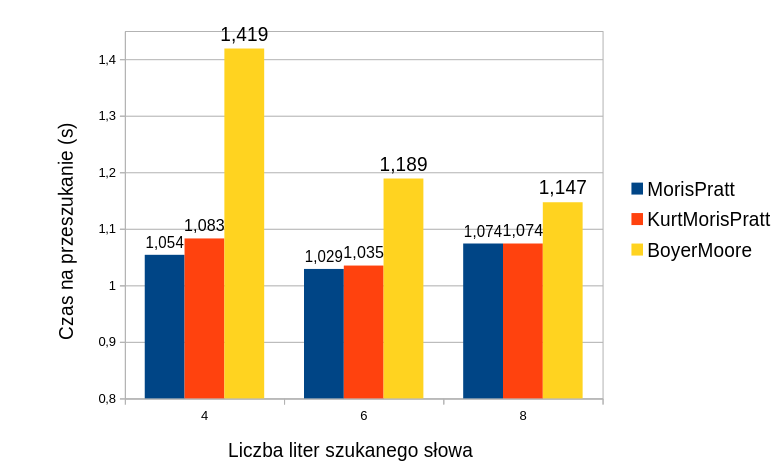
\includegraphics[width=\textwidth]{./images/GraphFirstAttempt.png}
    \caption{Wykres czasów bez statycznego bufora pliku oraz z ponowną 
    rekalkujacją bufora pre-procesora.}
    \label{fig:GraphFirstAttempt}
\end{subfigure}
%\hfill
\begin{subfigure}{0.8\textwidth}
    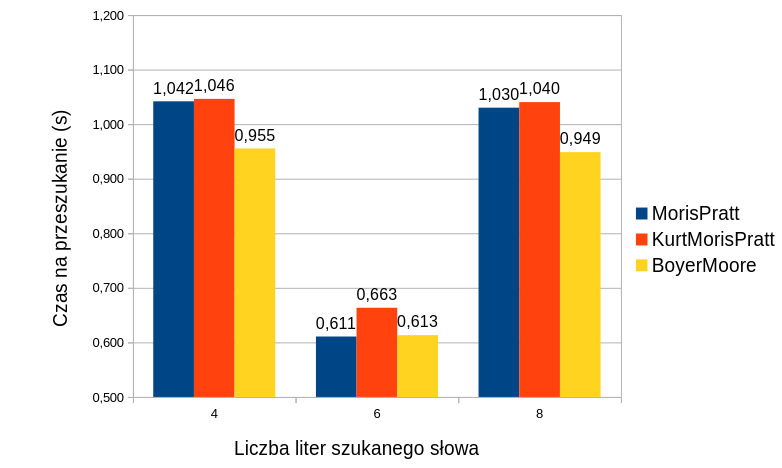
\includegraphics[width=\textwidth]{./images/GraphPreAllocBM.png}
    \caption{Wykres czasów bez statycznego bufora pliku z jednokrotną kalkulacją
     bufora pre-procesora dla algorytmu Boyer Moore'a. }
    \label{fig:GraphPreAllocBM}
\end{subfigure}
\begin{subfigure}{0.8\textwidth}
    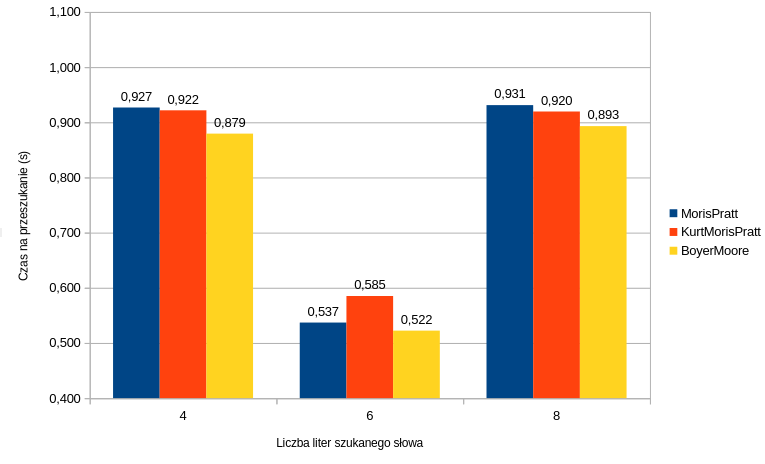
\includegraphics[width=\textwidth]{./images/GraphStaticPreallocAndFileBuffer.png}
    \caption{Wykres czasów z statycznym buforem pliku oraz statycznym buforem
    pre-procesora dla każdego algorytmu.}
    \label{fig:GraphStaticPreallocAndFileBuffer}
\end{subfigure}
\caption{Wykresy kolejnych iteracji na algorytmach}
\label{fig:GraphsIterationComparison}
\end{figure}

Pierwszy test wydajnościowy, który został przeprowadzony, sprawdzał wszystkie 
foldery, w których znajdowały się pliki. Za drugim razem ograniczono się tylko
do plików, które mogą posiadać oczekiwaną zawartość, odrzucając zatem część 
plików ze zbioru. Wykonano testy na 3 algorytmach, gdzie odczytywano 5191 plików 
i łącznie 240 MB danych. Oto rezultaty określonych algorytmów.

Algorytm Morisa-Pratta jest nieznacznie wolniejszy od algorytmu 
Kurta-Morisa-Pratta. Jest to spowodowane niewielką optymalizacją pomiędzy tymi 
dwoma algorytmami. Według danych na rysunku \ref{fig:GraphFirstAttempt} można 
zauważyć, KMP w niektórych przypadkach jest wolniejszy, niż algorytm MP, 
ponieważ posiada większe odchylenie standardowe, co powoduje, że jest mniej
stabilny. 


%Patrząc na statystki możemy zauważyć, że podczas pracy algorytmów, wystąpiły 
%wartości odstające (ang. \english{Outlier}) w niektórych wykonaniach dla 
%algorytmu KMP. Gdy usuniemy je pojawia się bardziej rzetelna informacja o 
%różnicy pomiędzy wynikami.

Algorytm Boyera-Moore'a wykorzystywany w takich narzędziach jak grep, posiada
wolniejszy czas egzekucji, co wynika z rys. \ref{fig:GraphFirstAttempt}, ale 
algorytm może zostać napisany w lepszy sposób. Z powodu implementacji, nie 
wykorzystywaliśmy ponownie bufora wcześniejszego procesowania, co wpływało na znaczne
spowolnienie algorytmu.

Implementacja, której wyniki widzimy na grafie \ref{fig:GraphFirstAttempt} jest
znacznie wolniejsza od pozostałych algorytmów. Powodem jest spędzanie znacznej
cześć czasu na stworzeniu tablicy wcześniejszego procesowania. Wiadome jest, że zawsze 
sprawdzamy ten sam ciąg we wszystkich plikach w folderze. Istnieje możliwość 
stworzenia tablicy wcześniejszego procesowania przy pierwszym użyciu algorytmu, a następnie
wykorzystanie tej tablicy we wszystkich odczytach.

Na następnym wykresie \ref{fig:GraphPreAllocBM} można zauważyć poprawę, gdy
implementacja algorytmu Boyer-Moora wykorzystuje ten sam bufor wcześniejszego procesowania, a
pozostałe algorytmy tworzą go od nowa, kiedy otwierany jest kolejny plik. Celem 
takiej implementacji było uzyskanie informacji o wpływie ponownego wykorzystania
bufora wcześniejszego procesowania na czas wykonania. 

Aby sprawdzić faktyczne wyniki, należało zaimplementować ponowne wykorzystanie
bufora wcześniejszego procesowania dla wszystkich algorytmów. Wyniki z drugiego wykresu 
potwierdziły wartość ponownego użycia bufora wcześniejszego procesowania w prędkości wykonania
algorytmu.

Ostatni wykres \ref{fig:GraphStaticPreallocAndFileBuffer} przedstawia implementację wykorzystującą ponownie bufor wcześniejszego
procesowania, jak i bufor przechowujący plik.
Bufor wcześniejszego procesowania był przydzielany przy każdym otwarciu nowego pliku,
co powodowało, że ten bufor mógł być zbierane przez \english{Garbage Collector}.
W przypadku użycia stałego bufora zapewniamy, że program nie będzie się pozbywał
bufora. Gdy na początku programu utworzymy bufor sami (nie polegając na optymalizacji języka),
algorytm Boyera-Moore'a odnotował 5 \% poprawę \ref{fig:GraphStaticPreallocAndFileBuffer}
w stosunku do poprzedniej implementacji.

Niestety statyczny bufor przechowujący plik, należy alokować, znając rozmiar 
największego pliku w folderze, który wynosił 11 MB. Było tak, gdyż odrzucaliśmy
obrazy. Moglibyśmy przed rozpoczęciem algorytmu sprawdzać rozmiar maksymalny 
pliku, ale to wydłuży czas działania. 

Istnieje też sytuacja, w której nie chcielibyśmy tego ograniczać, ponieważ nie
znamy największego pliku, a podanie zbyt małej ilość na bufor pliku spowoduje,
że nie otrzymamy poprawnych wyników, gdyż nie zmieści się on w całości do 
pamięci.

%\textbf{TODO porównanie wykorzystania pamięci (nie daje dużo info)}
